\section{Introduction}
One of the biggest challenges in the translation of neuroimaging findings into clinical practice is the need to validate models across large independent samples and across data obtained from different MRI scanners and sites. Combining multiple samples increases the overall sample size, overcoming a limitation common to many neuroimaging studies. However it also introduces heterogeneity into the sample from differences in scanner manufacturer, MRI protocol, variation in site thermal and power stability, as well as site differences in gradient linearity, centering and eddy currents. Therefore, images from different sites have the potential to introduce bias that can either mimic or obscure true changes or even worse, produce results that could be driven by the artifactual site differences. This can make the interpretation, reliability and reproducibility of findings difficult. Despite these issues, pooling data provides the opportunity to address a major source of concern regarding the low statistical power of published studies, especially when larger studies are not feasible due to financial constraints or recruitment is difficult because a particular disorder is rare at a specific geographical location \citep{poldrack2014making}.

Given the considerable incentives to pool data, there is a relative paucity of methods available to correct for site-specific differences in MR images. The majority of approaches are usually applied during data acquisition, for instance, using a common phantom across sites to calibrate and reduce differences in field homogeneities. However, these \textit{a priori} methods require careful planning and are not applicable to data sets that have already been collected or other \textit{post hoc} forms of data pooling. Site differences can also be addressed in a \textit{post hoc} fashion by treating the site as a covariate in the analysis for evaluation of confounding effects. However, the interaction between the usually unknown site-specific effects and the true brain effects on the MRI signal seem to be highly complex and nonlinear such that the inclusion of the covariate can also introduce bias \citep{rao2017predictive}.

Recent advances in computer vision due to the application of artificial neural networks suggests there may be a novel \textit{post hoc} solution  to remove non-linear bias in MR images. For example, superior performance in non-linear, multivariate pattern classification problems such as Alzheimer’s disease classification, brain lesion segmentation, skull stripping and brain age prediction have been achieved using deep learning networks \citep{payan2015predicting, sarraf2016deepad, kamnitsas2017efficient, kleesiek2016deep, cole2017predicting}. Deep learning provides some unique advantages for high-dimensional data such as MRI data, since it does not require extensive feature engineering. Furthermore, deep learning has produced important advances in generative modeling. Generative modeling involves learning to estimate a given distribution in order to produce examples from that distribution. For example, after being trained on a set of images, the model is able to generate a new, `unseen’ sample from the training set. Generative modeling is considered a much more difficult task than pattern classification, as the output of these models are typically high dimensional and a single input may correspond to many correct answers (e.g. there are many ways of producing an image of a cat).

One class of generative models, known as generative adversarial networks (GANs), have recently achieved considerable success in a variety of image problems, from image generation \citep{radford2015unsupervised}, super resolution generation \citep{ledig2016photo}, text2image \citep{reed2016generative} and image-to-image translation \citep{isola2016image} (See Figure \ref{fig:cycle_gan} for examples). GANs succeed through the idea of adversarial training, where the model’s training process can be described as a game between two players. One player is called the generator where it attempts to create samples from the same distribution as the observed data. The other player is the discriminator where its function is to examine the fake samples from the generator and real samples from the observed data and to classify the generated and observed samples as either real or fake. Over time, the discriminator is trained with supervision to better distinguish real and fake samples. However at the same time, the generator will improve its synthesis of fake samples in order to fool the discriminator, which in turn will make the job of the discriminator more difficult. Eventually the solution of this game is a Nash equilibrium, where the generator is unable to improve its generation of fake samples and the discriminator is unable to better classify real and fake samples \citep{goodfellow2016nips}. See Box 1 for further details.

\begin{figure}[htp]
\begin{center}
 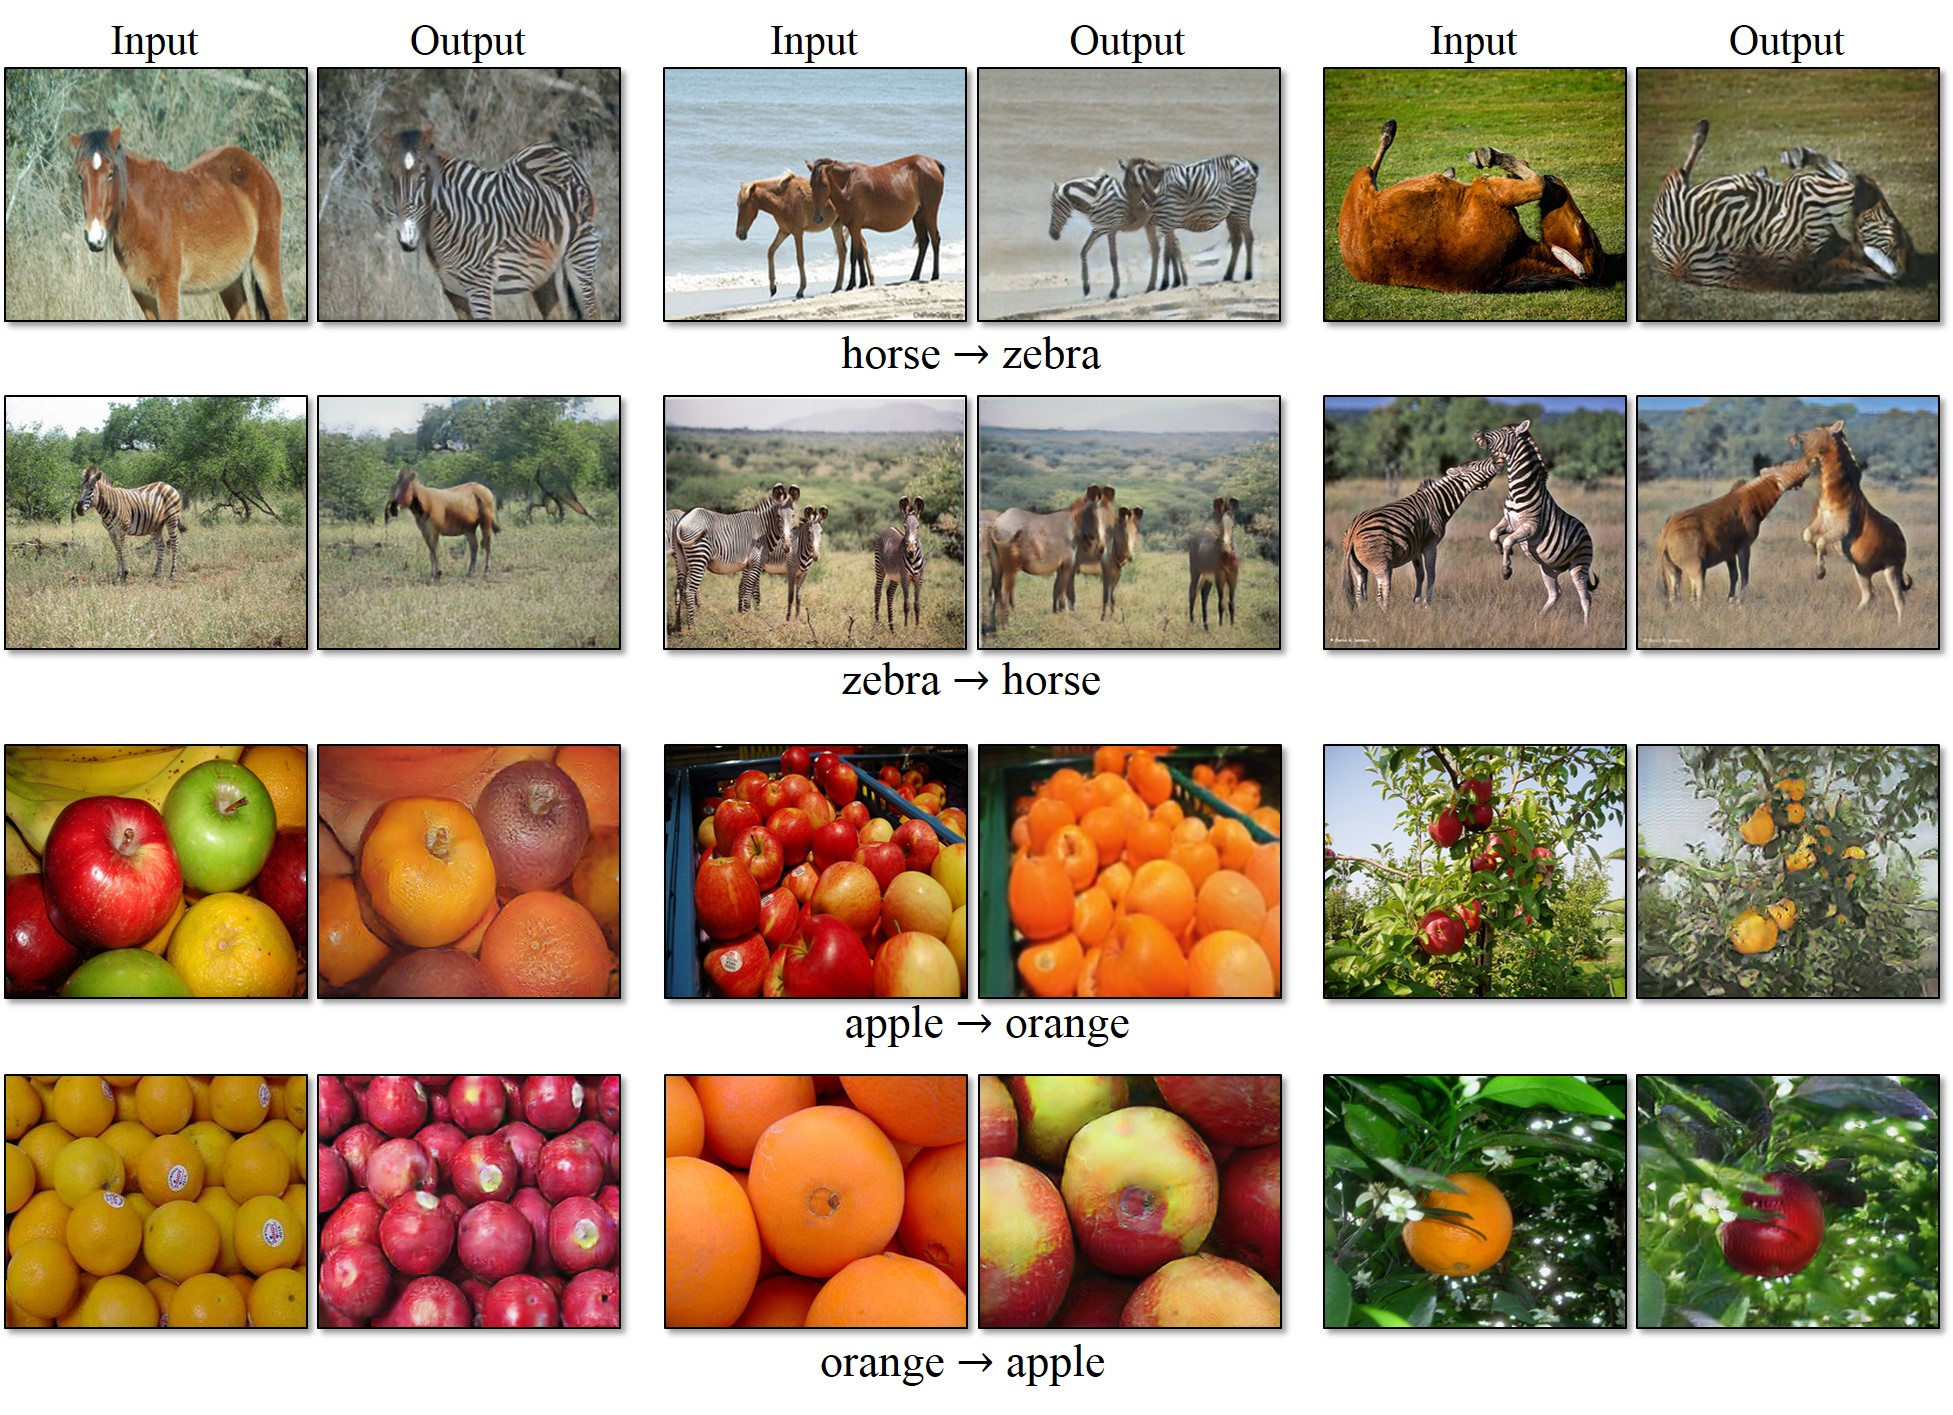
\includegraphics[width = 0.9\textwidth]{objects.jpg}
    \end{center}
  \caption{Examples of images produced from CycleGAN. Reproduced from  \cite{zhu2017unpaired} without adaption, under CC-BY 4.0 }
  \label{fig:cycle_gan}
\end{figure}

Here, we propose an algorithm that uses GANs to transform a set of images from a given MRI site into images with characteristics of a different MRI site. Its purpose is to correct for differences in site artifacts without the need for \textit{a priori} calibration using phantoms or significant coordination of acquisition parameters. This algorithm can be treated as a ’black box’ without knowledge of the artifacts present in the dataset and can be applied \textit{post hoc} after acquisition to two or more unpaired sets of imaging data. Importantly, as we demonstrate, the correction occurs without any apparent loss of information related to gender or clinical diagnosis.
